\section{Experiments}
\label{experiments}
In mobile voice manipulation applications and in found data cases, it is mandatory to use audio recorded far from the ideal studio conditions, with the possibility of finding background noise.
%
Nevertheless, in some vocoding and adaptation techniques noise present in the adaptation data can add background noise and produce distortion in the synthetic speech signal.

A GlottHMM-based speaker-adaptive statistical speech synthesis is built in this project, testing the effects of using noisy data in the adaptation.
%
The different noises included in the adaptation data are: babble noise, factory noise and machine gun noise, with different signal-to-noise ratio (SNR).
%
These noises where artificially added into clean data.
%
The results will be compared to the ones obtained with the STRAIGHT-based system in \cite{karhila_jstsp_14}.

From now on, we will refer to noise reduction configuration as the one set by the parameter values shown in Appendix \ref{glott_conf_noise_red} (set to true).

\subsection{Initial Experiments}
\label{experiments_initial}
The use of glottal pulses for HMM-synthesis was originally proposed due to the buzzy voice quality caused by simple excitation \cite{raitio2008hmm}.
%
However, a proper modelling of the glottal pulse shape improves the quality in the case of lower fundamental frequency speakers. On the other hand, speakers with higher $F_{0}$, such as women, do not benefit from the pulse and the impulse excitation may be adequate for them.
%
This particular behavior is the reason of working with a male average voice model, knowing that glottal inverse filtering approach flaws when synthesizing high-pitched voices.

The first step is testing the performance in analysis-resynthesis of GlottHMM when noisy data is used, in order to see if the performance of GlottHMM degrades when background noise is present in the samples. This is done using the analysis and synthesis modules of GlottHMM.

\begin{figure}[!htb]
\begin{centering}
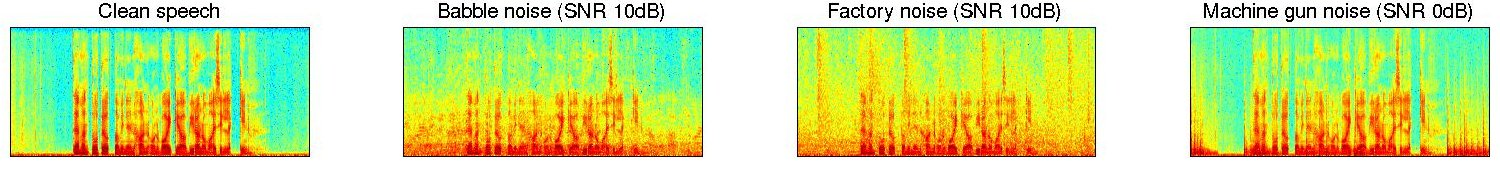
\includegraphics[width=\textwidth]{images/natural_spectra.jpg}
\caption{Natural speech FFT spectra of clean speech, speech with babble noise, factory noise and machine gun noise}
\label{fig:natural_spectra}
\end{centering}
\end{figure}

Figure \ref{fig:natural_spectra} shows the spectra of a natural speech sample in different environmental conditions while Figure \ref{fig:synthetic_spectra} shows the spectra of the same samples resynthesized with GlottHMM.

\begin{figure}[!htb]
\begin{centering}
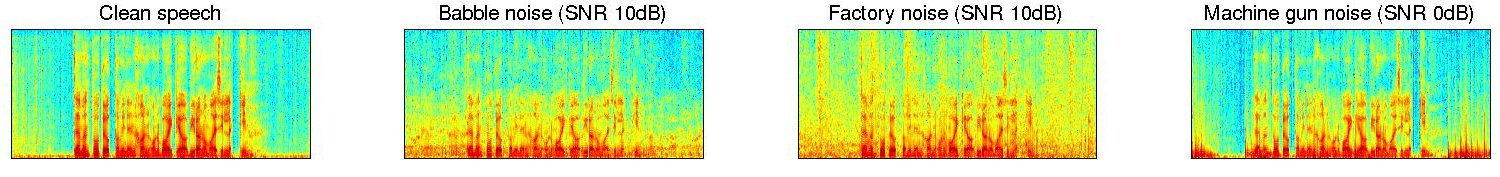
\includegraphics[width=\textwidth]{images/synthetic_spectra.jpg}
\caption{Synthetic speech FFT spectra of clean speech, speech with babble noise, factory noise and machine gun noise after analysis and resynthesis with GlottHMM}
\label{fig:synthetic_spectra}
\end{centering}
\end{figure}

As it can be seen, both the natural and the synthetic spectra have little differences between them.
%
%
After listening to the samples we could conclude that noise was not influencing the regular performance GlottHMM more than it influenced the performance of STRAIGHT in the experiments carried out in \cite{karhila_jstsp_14}.

Another important issue is finding a correct configuration for GlottHMM.
%
In Appendix \ref{glott_conf_file}, the configuration file needed by GlottHMM can be found.
%
As it can be seen, this file has a great amount of options to configure. 
%
However, thanks to previous experiments conducted and the advice of Tuomo Raitio, who developed GlottHMM, the tweaks to make in the configuration file are focused in noise robustness and some voice characteristics.

Some low $F_{0}$ problems were noticed during the first rounds of experiments.
% 
This problems consisted of frames where the voice sounded funny.
%
To find out the details of this issue, a simple $F_{0}$ histogram plotting was made.
%
Figure \ref{fig:f0_histograms} presents the histograms of the voices used to build the average voice model, where low-frequency peaks can be pointed out in some of the voices.

\begin{figure}[!htb]
\begin{centering}
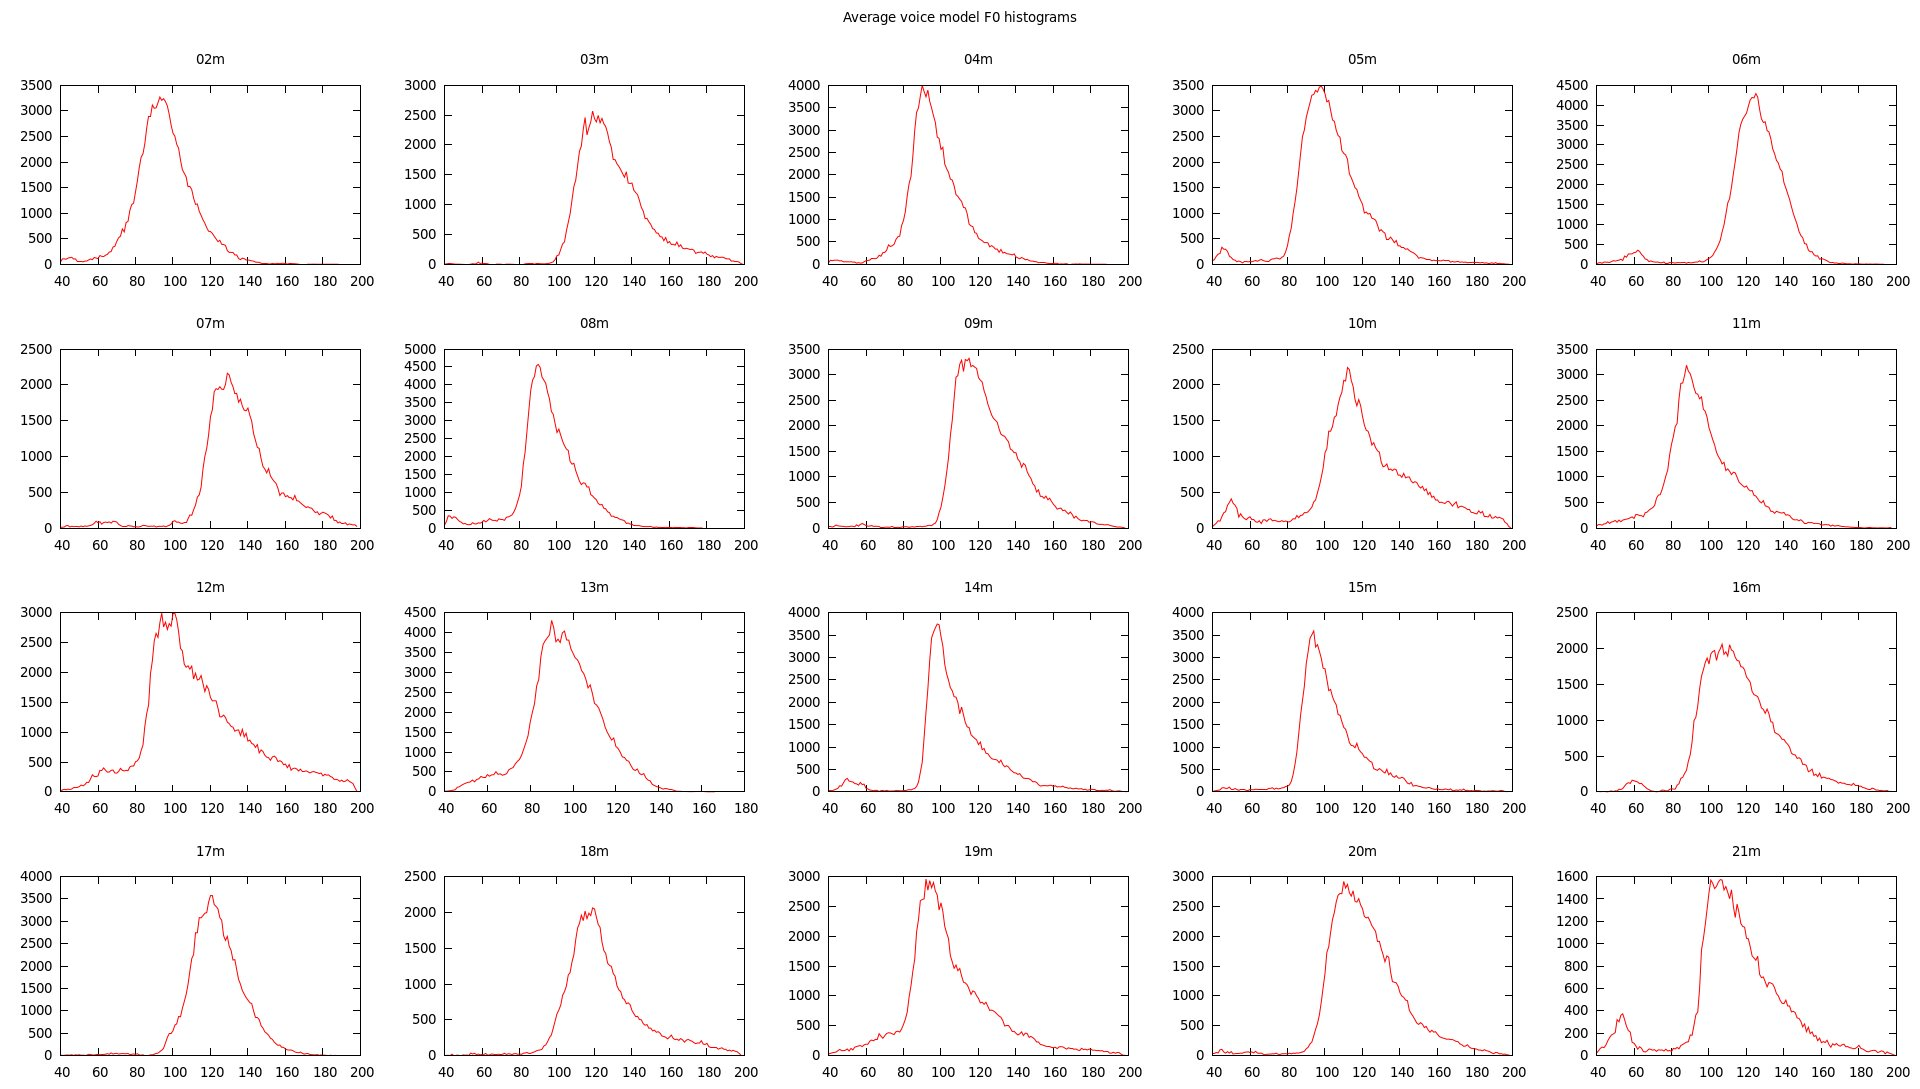
\includegraphics[width=\textwidth]{images/av_model_=conf_f0_histogram.jpg}
\caption{Histogram of the $F_{0}$ values of individual frames from the voices composing the average voice model, extracted with no lower or upper bounds}
\label{fig:f0_histograms}
\end{centering}
\end{figure}

Solving this problem only required to extract again the features for the voices with low-frequency peaks.
%
These peaks were found around 40-60 Hz in the training data, used in the average voice model, and in the adaptation data.
%
To eliminate them, in the configuration file the $F_{0}$ lower-limit was set to 65 Hz.

The last round of initial experiments conducted aim to find the best combination of the noise reduction parameters shown in Appendix \ref{glott_conf_noise_red}.
%
These experiments consist on analysis and resynthesis of the noisy data varying the parameters in Appendix \ref{glott_conf_noise_red} and carrying out the objective measures described in \ref{evaluation_objective}.
%

\begin{figure}[!htb]
\begin{centering}
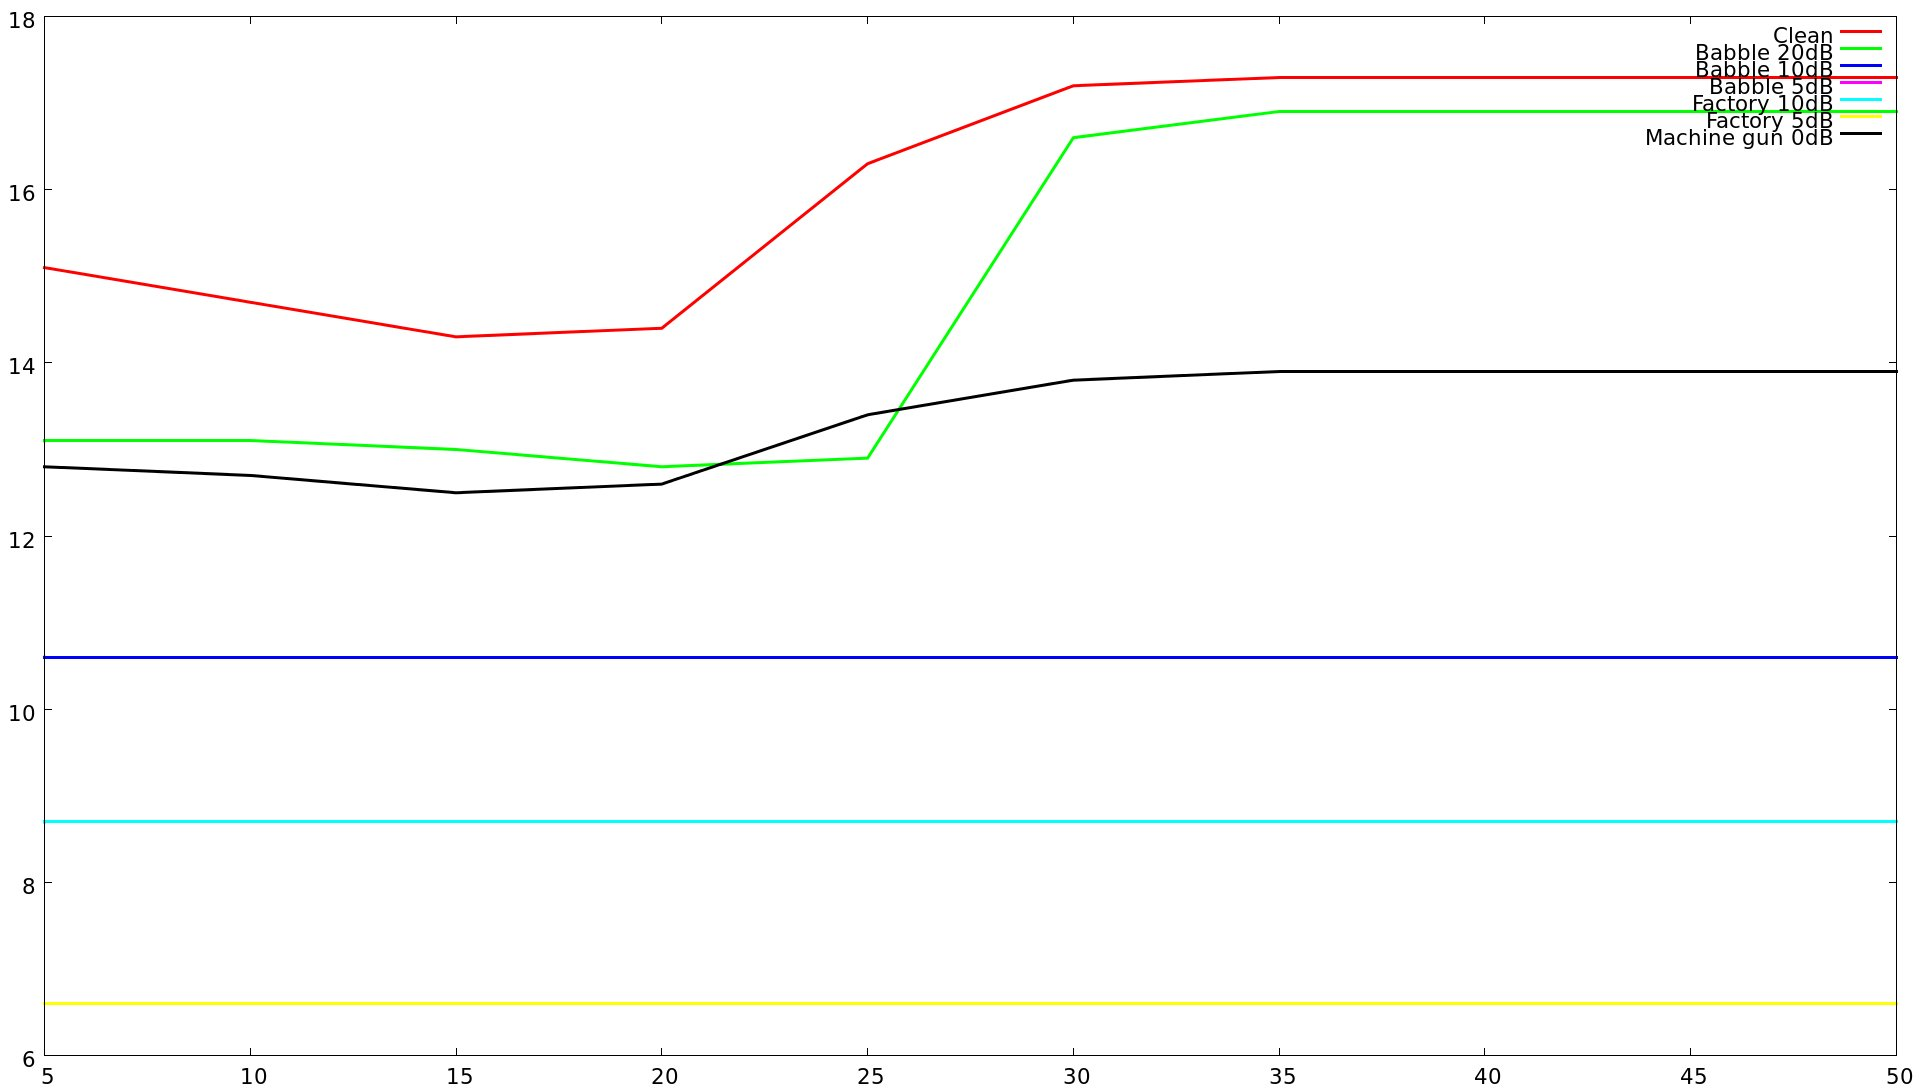
\includegraphics[width=\textwidth]{images/noise_red_snr_exp.jpg}
\caption{SNR measures with $NOISE\_REDUCTION\_LIMIT = 4.5$ fixed and $NOISE\_REDUCTION\_DB$ from 5 to 50}
\label{fig:noise_red_snr}
\end{centering}
\end{figure}

\begin{figure}[!htb]
\begin{centering}
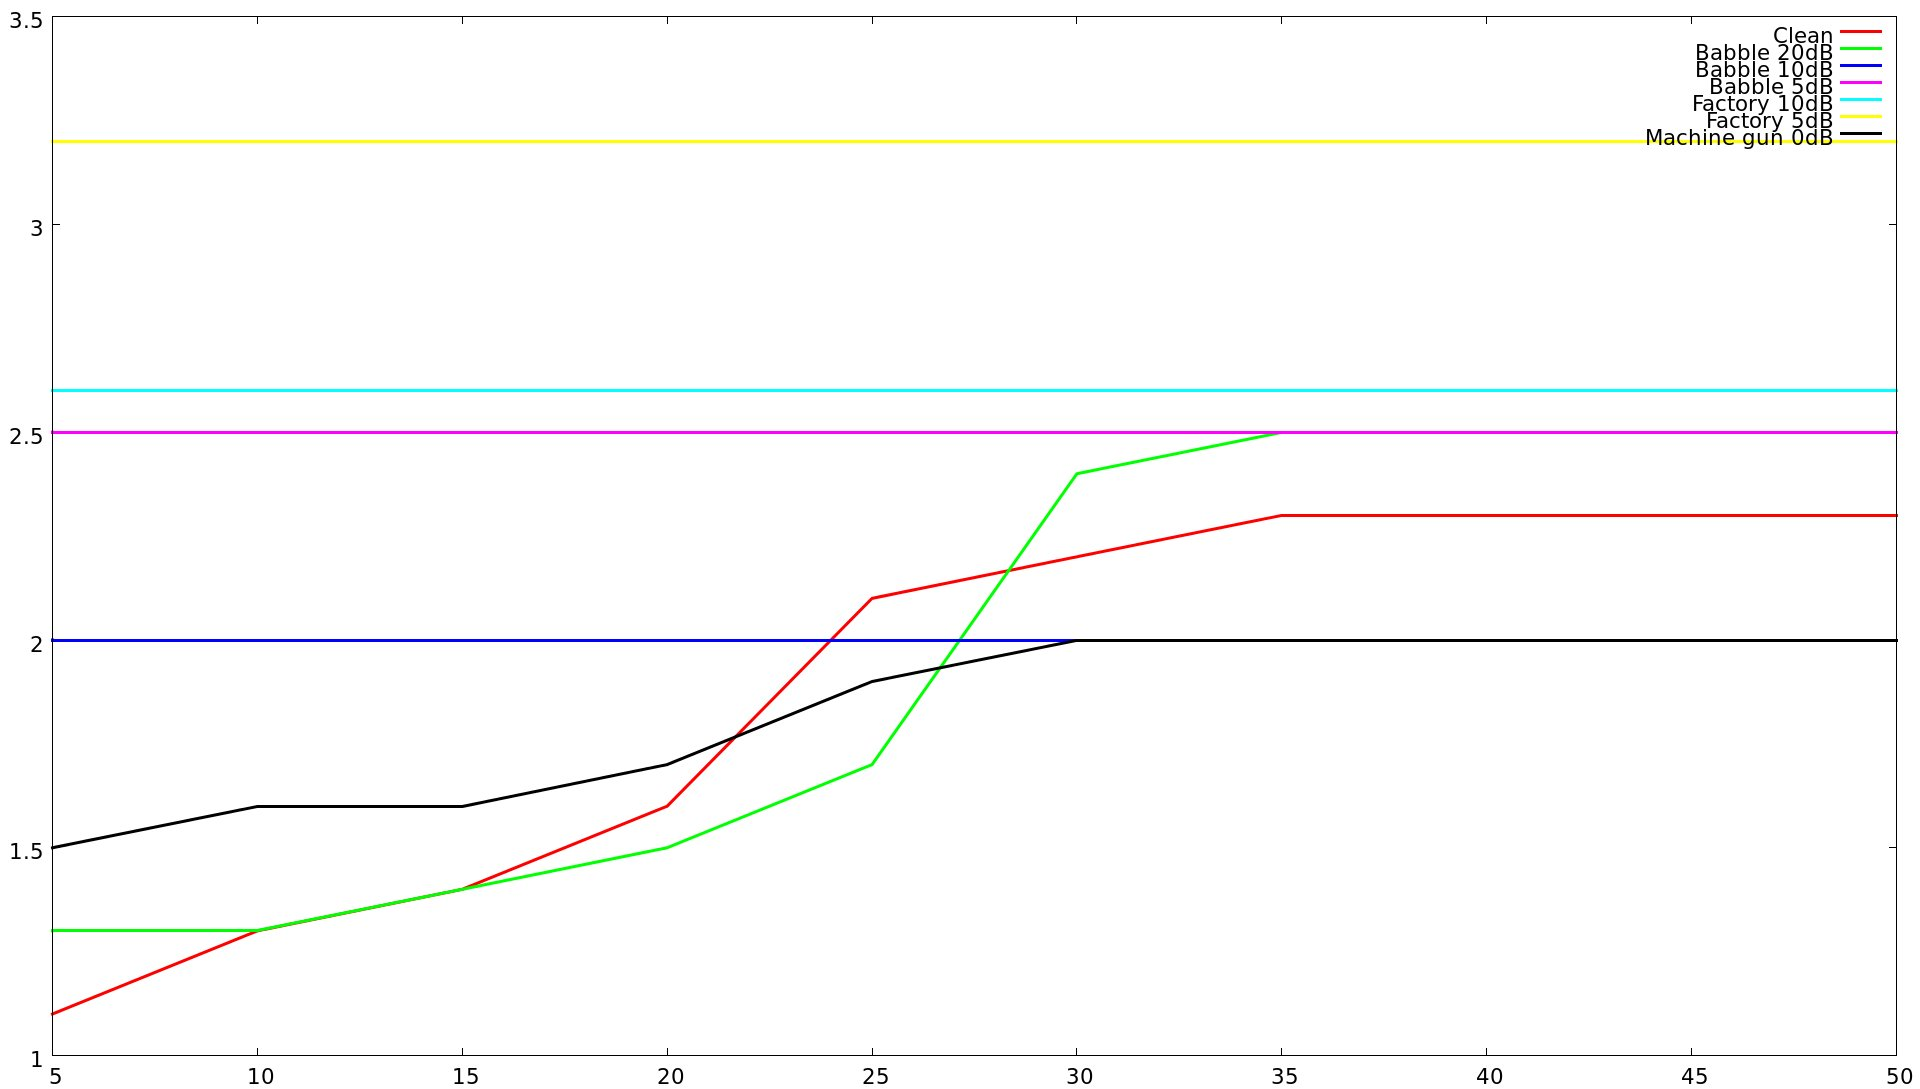
\includegraphics[width=\textwidth]{images/noise_red_mcd_exp.jpg}
\caption{MCD measures with $NOISE\_REDUCTION\_LIMIT = 4.5$ fixed and $NOISE\_REDUCTION\_DB$ from 5 to 50}
\label{fig:noise_red_mcd}
\end{centering}
\end{figure}

\begin{figure}[!htb]
\begin{centering}
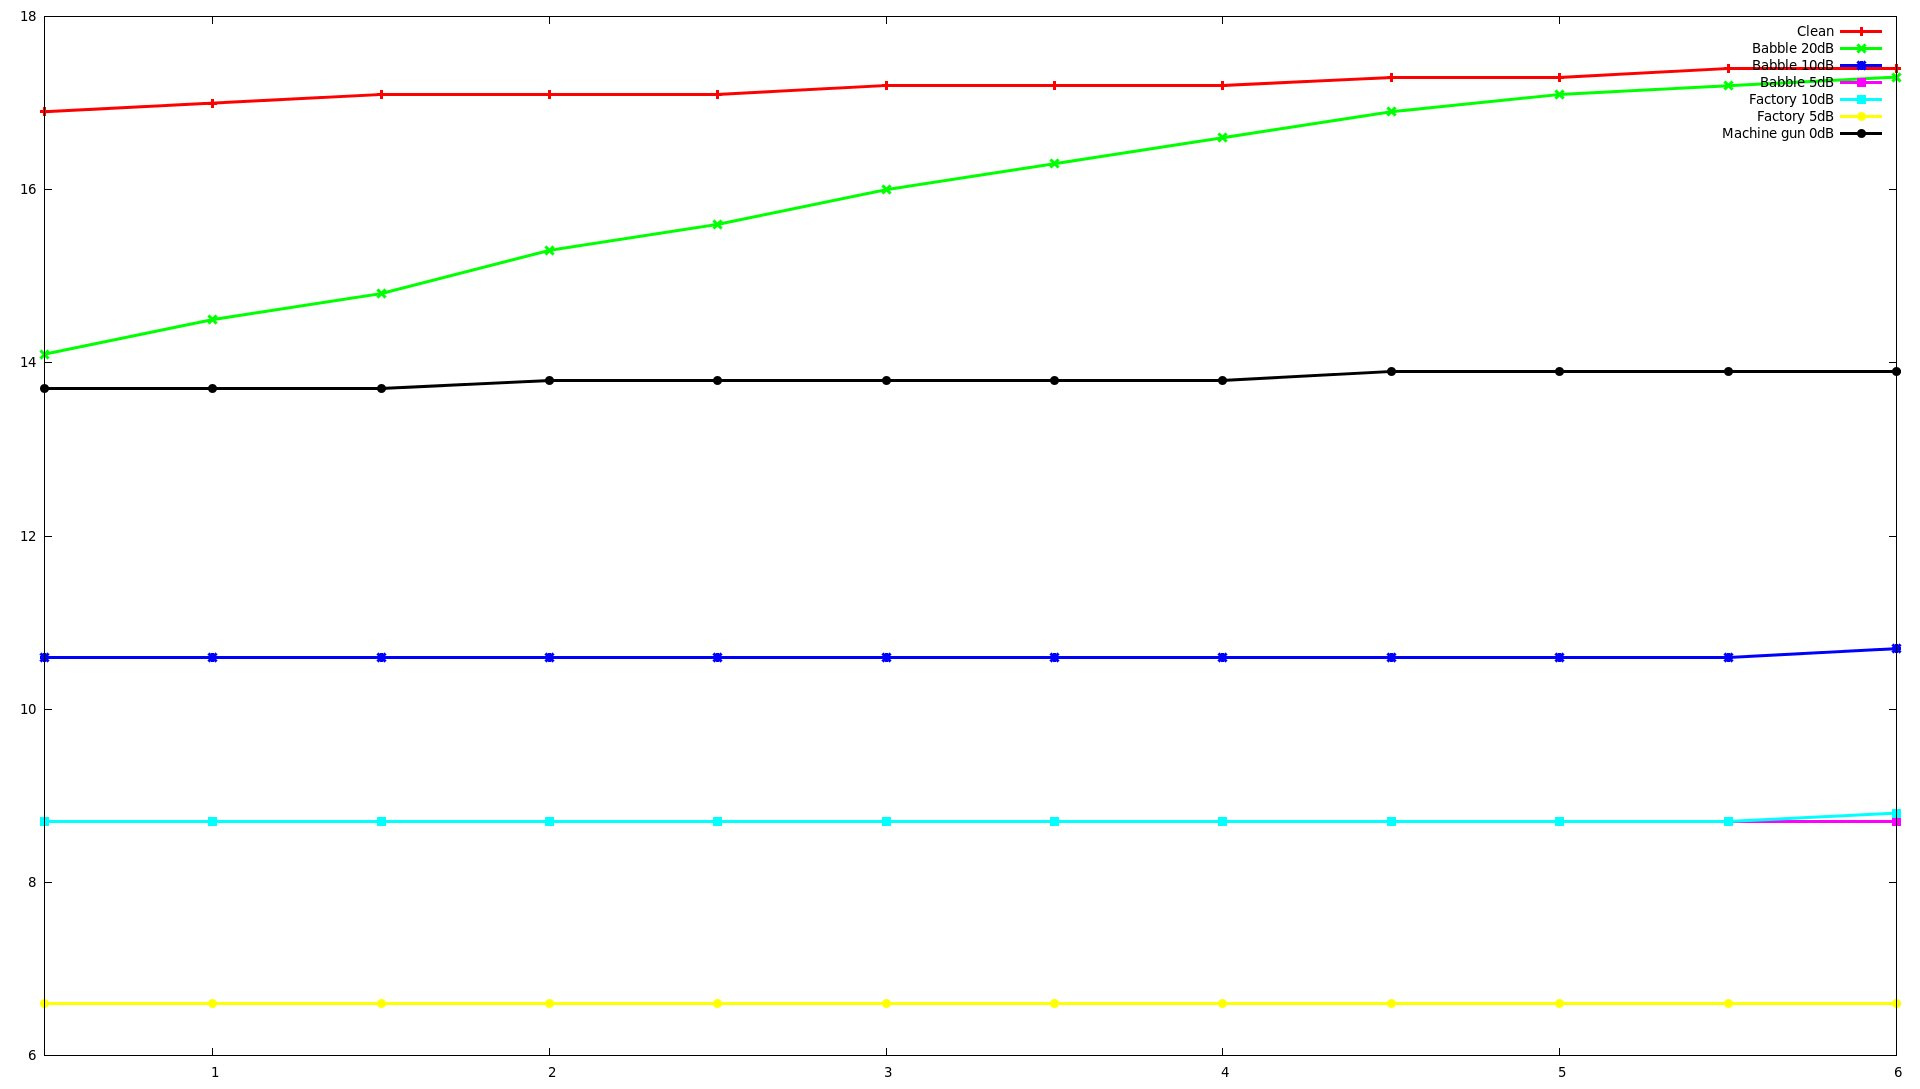
\includegraphics[width=\textwidth]{images/noise_red_lim_snr_exp.jpg}
\caption{SNR measures with $NOISE\_REDUCTION\_DB = 35$ fixed and $NOISE\_REDUCTION\_LIMIT$ from 0.5 to 6}
\label{fig:noise_red_lim_snr}
\end{centering}
\end{figure}

\begin{figure}[!htb]
\begin{centering}
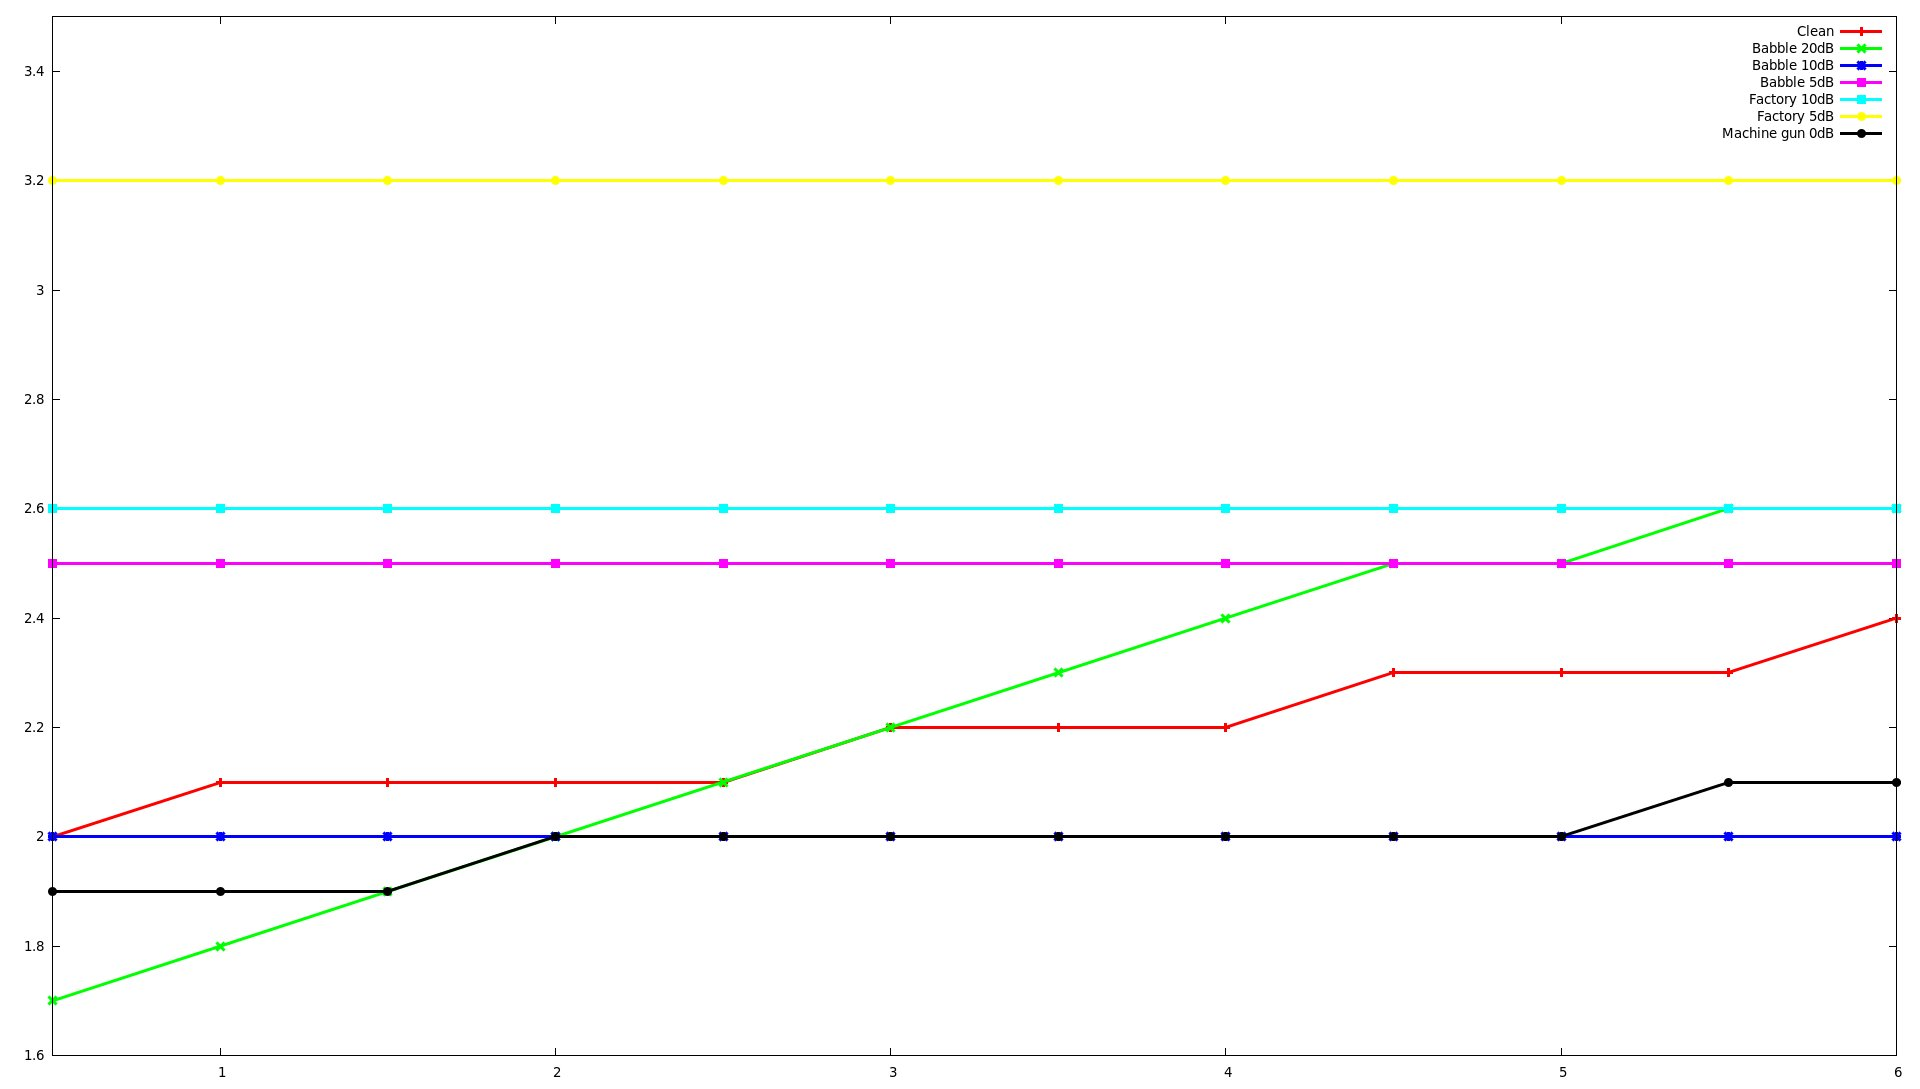
\includegraphics[width=\textwidth]{images/noise_red_lim_mcd_exp.jpg}
\caption{MCD measures with $NOISE\_REDUCTION\_DB = 35$ fixed and $NOISE\_REDUCTION\_LIMIT$ from 0.5 to 6}
\label{fig:noise_red_lim_mcd}
\end{centering}
\end{figure}
Figures \ref{fig:noise_red_snr}, \ref{fig:noise_red_mcd}, \ref{fig:noise_red_lim_snr} and \ref{fig:noise_red_lim_mcd} illustrate the evolution of the SNR and MCD measures when varying NOISE\_REDUCTION\_DB with a fixed NOISE\_REDUCTION\_LIMIT and vice versa.
%
As it can be seen in Figure \ref{fig:noise_red_snr}, for a fixed noise reduction limit the SNR measures increase significantly (higher SNR scores mean better quality) between 20 and 35dB noise reduction for the cases of clean and babble 20dB samples, reaching a limit.
%
Also, there is a slight improvement in the case of machine gun 0dB noise, but in the rest of the cases no improvement is seen.
%
As SNR scores increase MCD follows a similar patter (higher MCD scores mean worse quality).
%
In Figure \ref{fig:noise_red_mcd} it can be seen that the cases where the SNR was increasing are the ones with an increase of the MCD scores.
%
The ones with steady SNR scores have no changes in the MCD either.

The case where NOISE\_REDUCTION\_DB is fixed and the variation is made in the NOISE\_REDUCTION\_LIMIT is presented in Figures \ref{fig:noise_red_lim_snr} and \ref{fig:noise_red_lim_mcd}.
%
When increasing the NOISE\_REDUCTION\_LIMIT a steady increase of the SNR scores is only appreciable in the case of babble 20dB background samples.
%
All the other cases remain stable, although a very small increase, not significant, can be spot for clean and machine gun 0dB cases.
%
MCD scores follow the same pattern explained before. 
%
Babble 20dB has both increases in SNR and MCD.
% 
Not so big as in babble 20dB case increases in MCD can be found also for the clean and machine gun cases, probably due to the small improvement appreciated in their SNR.

A frame by frame representation of the natural waveform, resynthesized waveforms and SNR and MCD measures for the cases of babble 10dB and 20 dB background noise is shown in Figures \ref{fig:frame_by_frame_babble10} and \ref{fig:frame_by_frame_babble20}.

\begin{figure}[!htb]
\begin{adjustwidth}{-2.6cm}{}
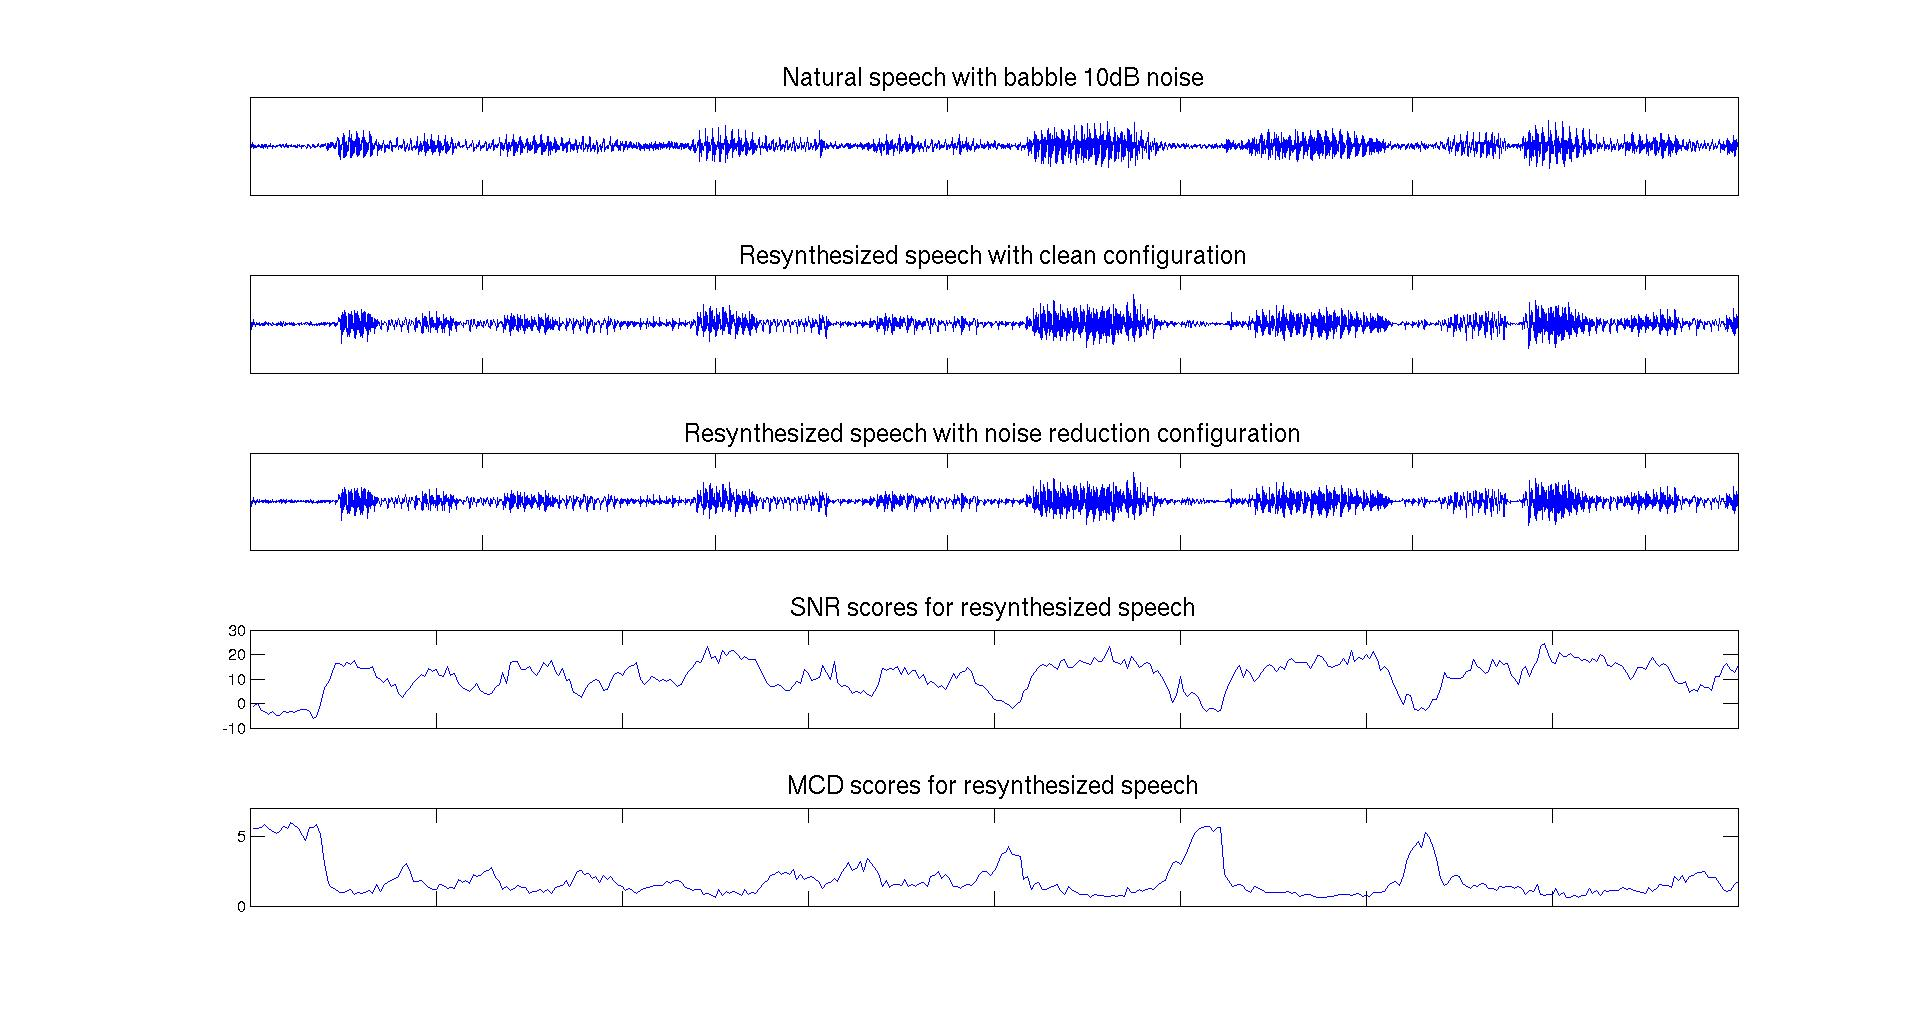
\includegraphics[width=1.3\textwidth]{images/babble10_frame_by_frame.jpg}
\end{adjustwidth}
\caption{Frame by frame representation of the natural speech with a babble background noise level of 10dB, resynthesized speech after analysis with GlottHMM not using the noise reduction module values in Appendix \ref{glott_conf_noise_red} (set to true), resynthesized speech using the noise reduction module and SNR and MCD measures for the last synthetic sample}
\label{fig:frame_by_frame_babble10}
\end{figure}

\begin{figure}[!hb]
\begin{adjustwidth}{-2.6cm}{}
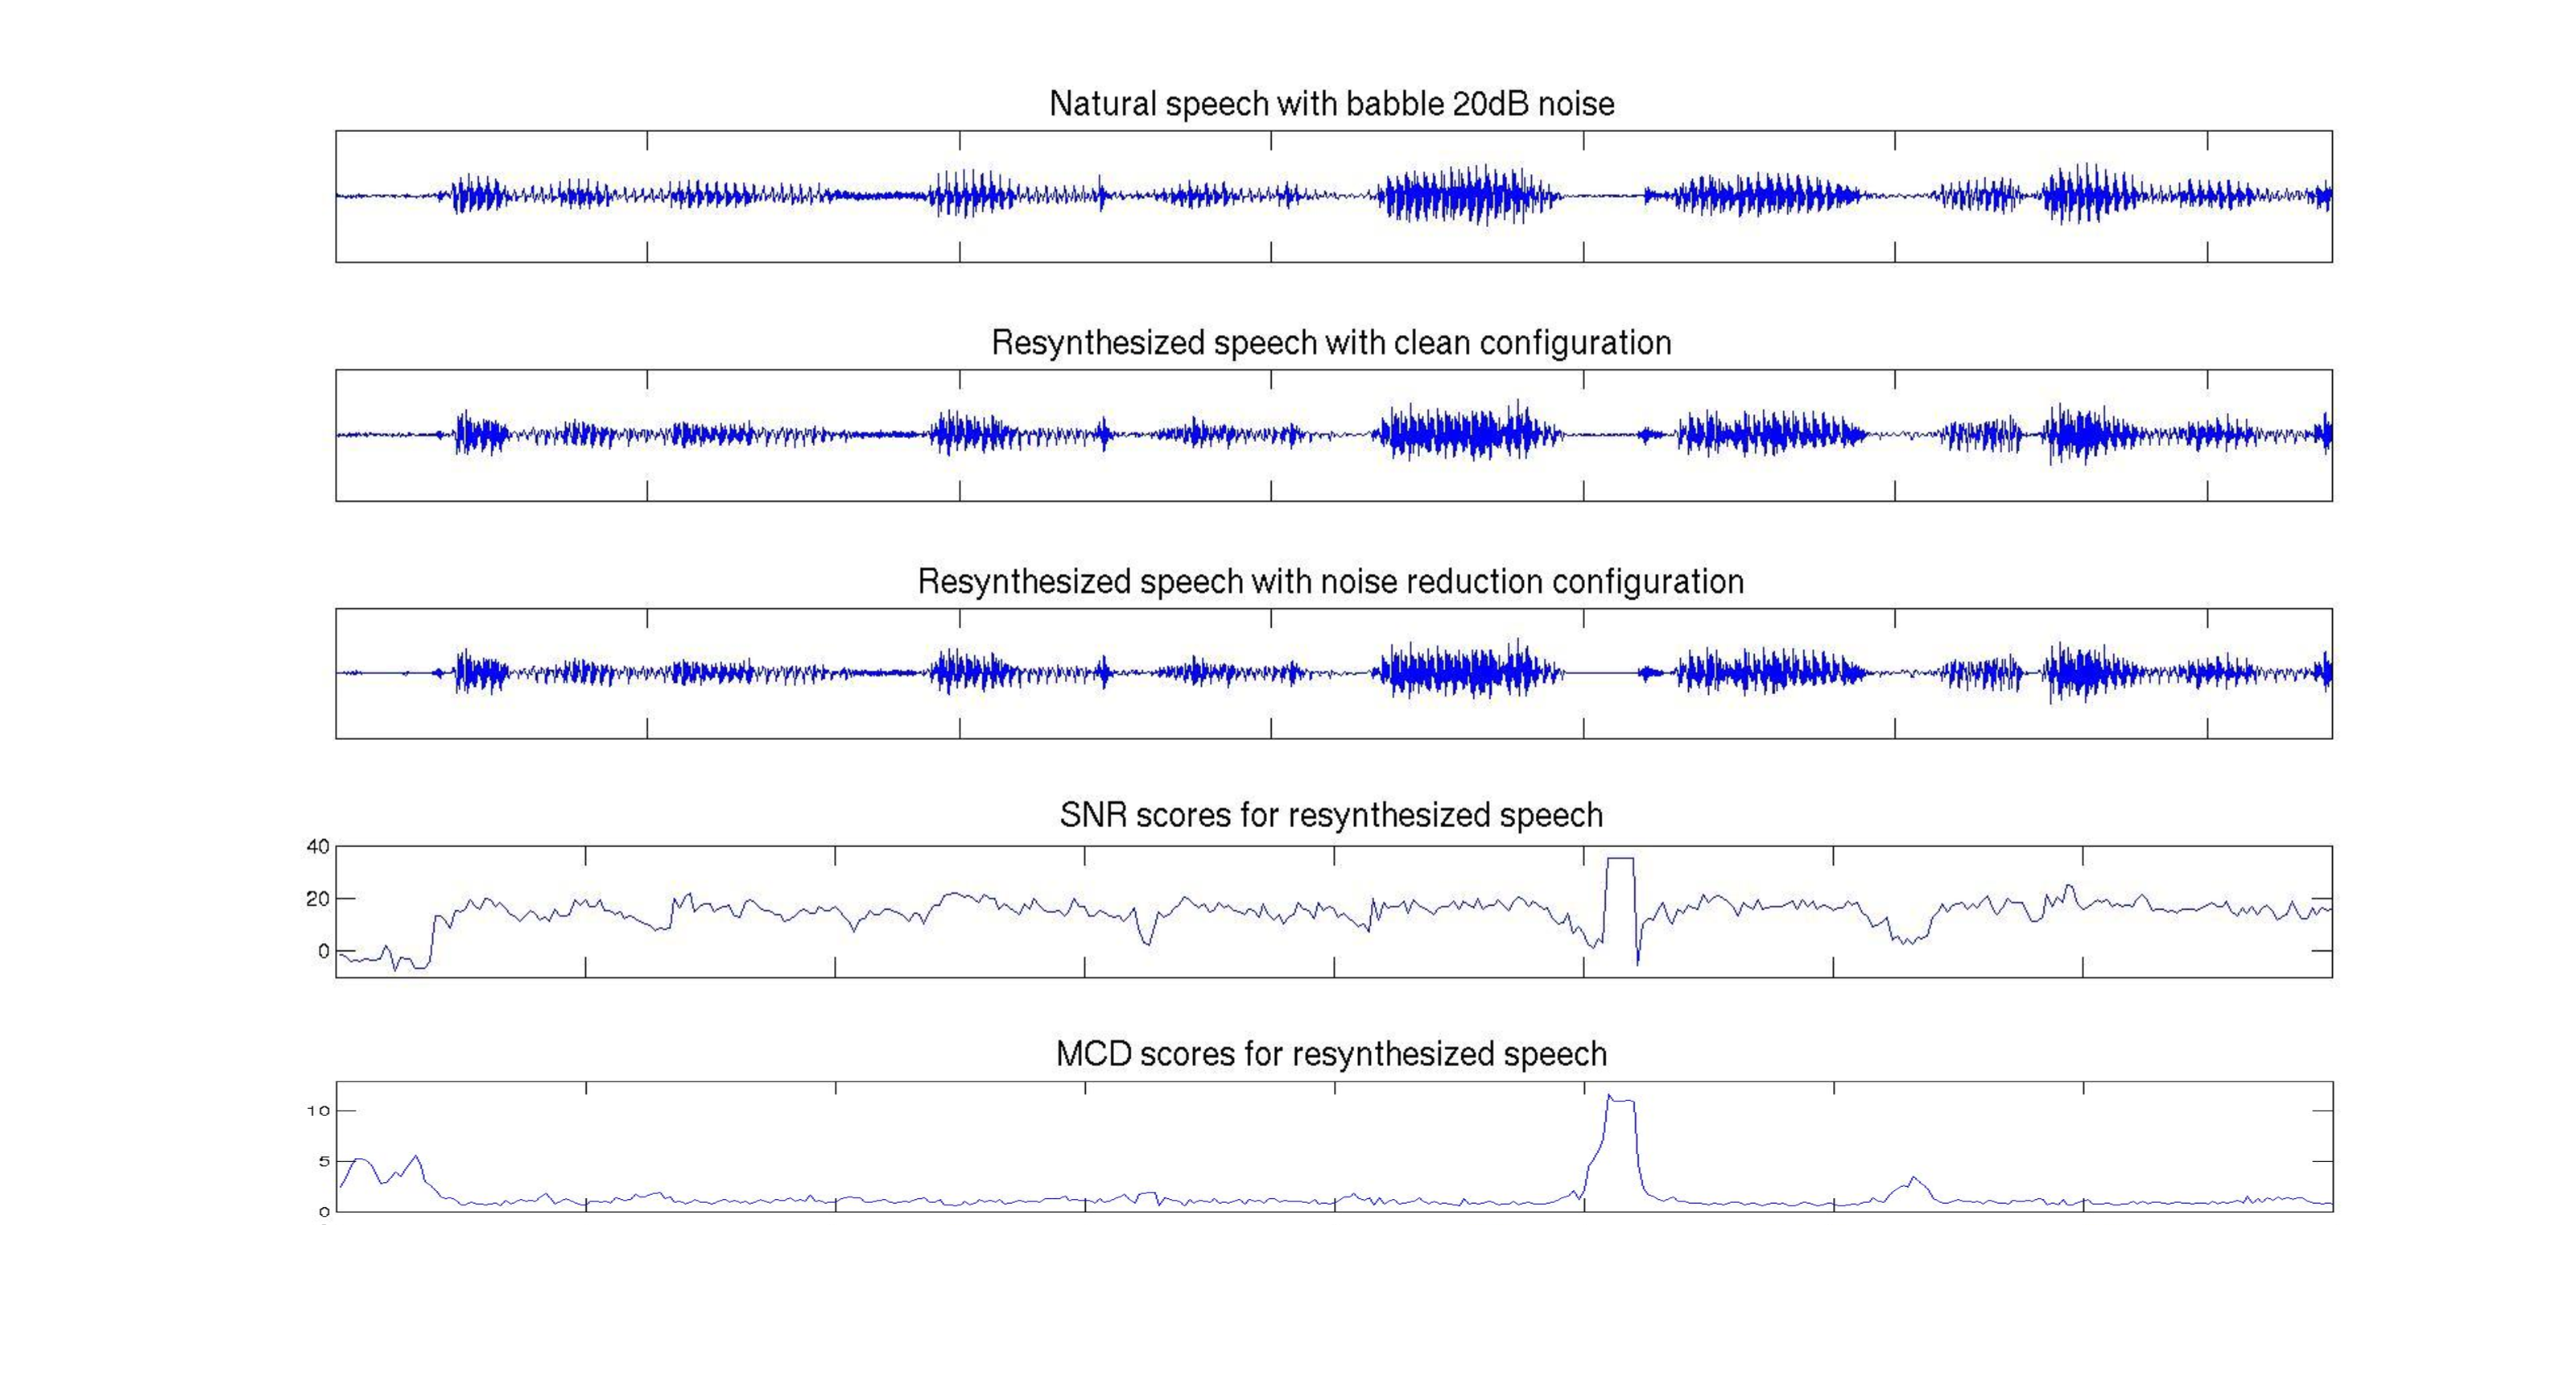
\includegraphics[width=1.3\textwidth]{images/babble20_frame_by_frame.pdf}
\end{adjustwidth}
\caption{Frame by frame representation of the natural speech with a babble background noise level of 20dB, resynthesized speech after analysis with GlottHMM not using the noise reduction module values in Appendix \ref{glott_conf_noise_red} (set to true), resynthesized speech using the noise reduction module and SNR and MCD measures for the synthetic samples}
\label{fig:frame_by_frame_babble20}
\end{figure}

In the case of the waveforms, we can see no difference when the data is corrupted with a 10dB level babble noise, while when the background noise level is 20dB the noise reduction module used by GlottHMM results in an improvement of the quality attending to cleaner synthetic waveform in speech silences and better objective measures, visible for example when the SNR reaches its maximum value (35 dB). 

A comparison between the measures done when resynthesizing using the noise reduction module and without using it is shown in Figures \ref{fig:babble10_clean_vs_noise} and \ref{fig:babble20_clean_vs_noise}. 
%
No significant difference can be spotted when talking about the babble 10dB case.
%
Nevertheless, in the case of having a babble 20dB background noise, we can point out different frames where the noise reduction module is clearly improving the SNR quality (careful with the different scales in the graph).
%
Some frames reach the maximum SNR value (35 dB) while when not using the noise reduction module the same frames form a valley in the SNR graph.
%
Other examples of this behavior can be found at the graph.

However, the MCD measures in those cases are contradictory. 
%
While the SNR increases, meaning a quality improvement, the MCD also increases creating the opposite effect, a quality decrease.
%
This behavior has been noticed in the silences present along the utterance.

From all these initial experiments it can be said that the noise reduction included in the GlottHMM vocoder is not capable of carrying out its function when severe noise conditions are found.
%
However, when the noise conditions are reasonable to record audio, these first experiments show that GlottHMM gets along quite well in analysis and resynthesys, potentially improving the quality when adapting an HMM-based system. 

\begin{figure}[!htb]
\begin{adjustwidth}{-2.6cm}{}
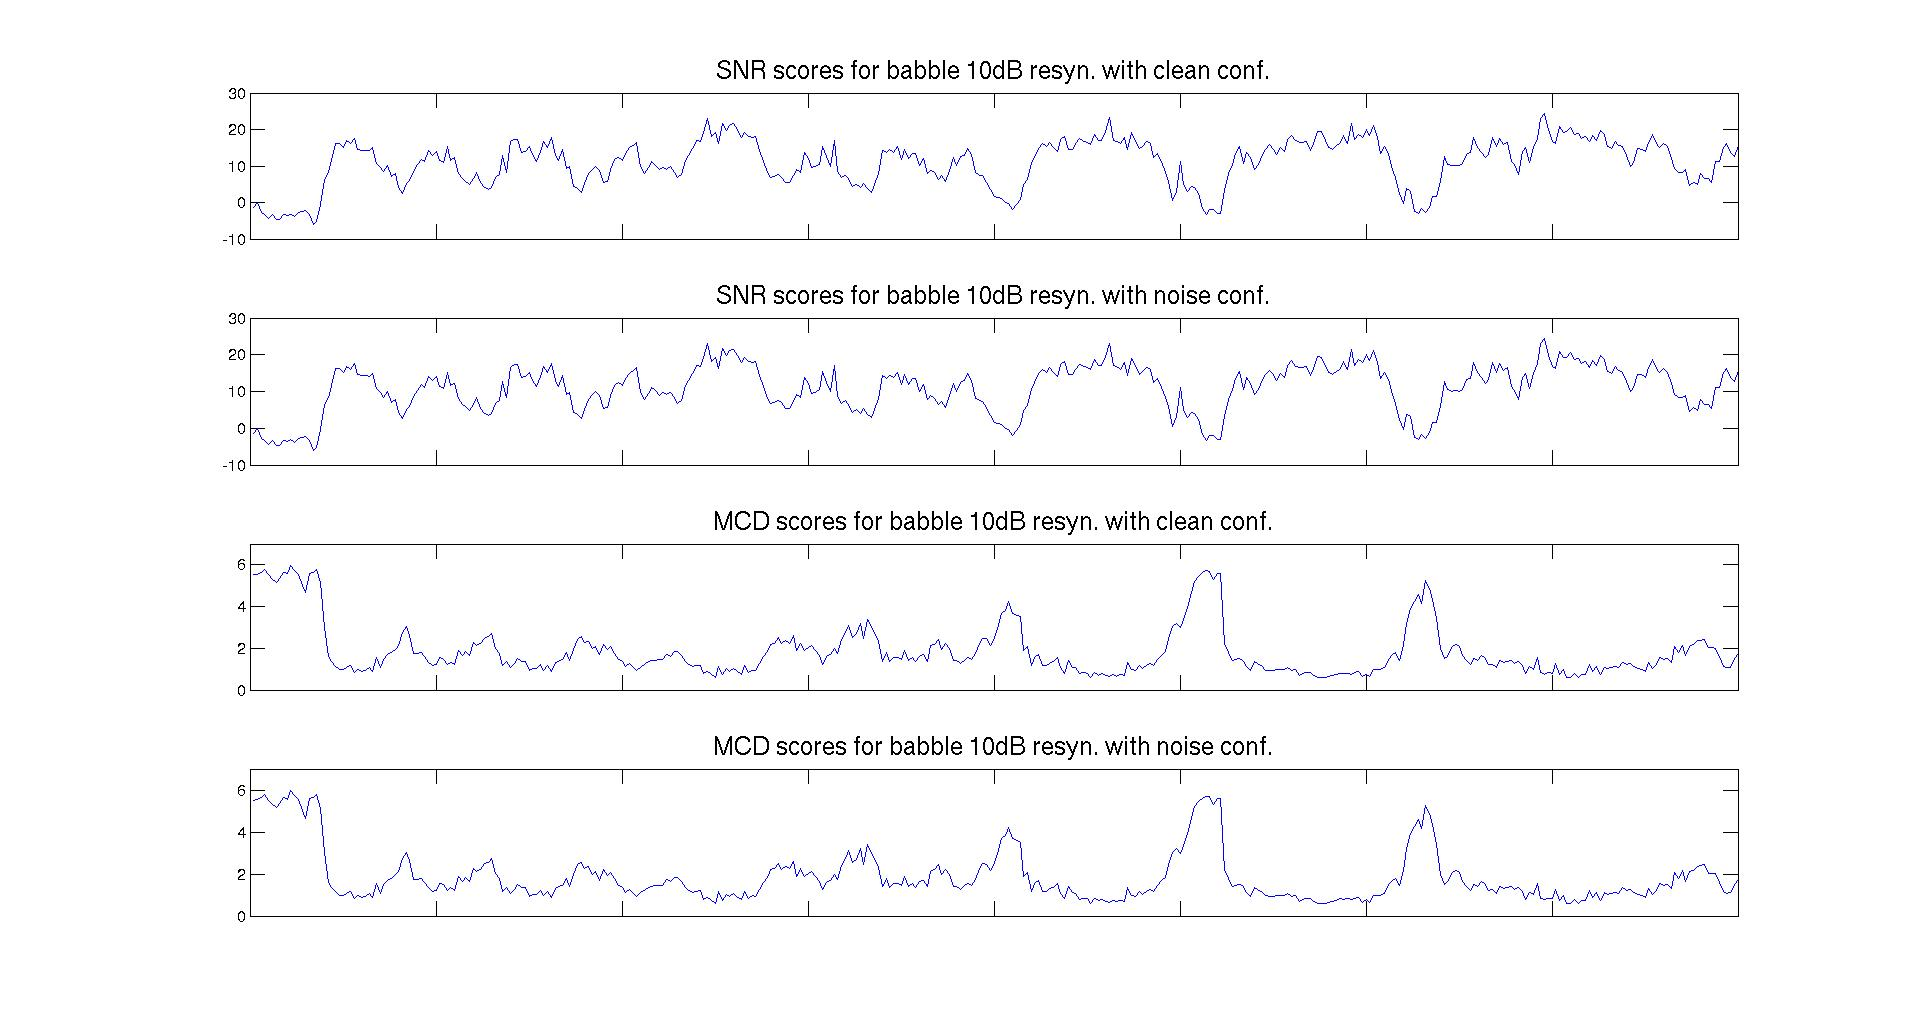
\includegraphics[width=1.3\textwidth]{images/babble10clean_vs_noise.jpg}
\end{adjustwidth}
\caption{SNR and MCD measures of a resynthesized sample with babble 10dB background noise using and not using the noise reduction module (values in Appendix \ref{glott_conf_noise_red}, set to true)}
\label{fig:babble10_clean_vs_noise}
\end{figure}

\begin{figure}[!hb]
\begin{adjustwidth}{-2.6cm}{}
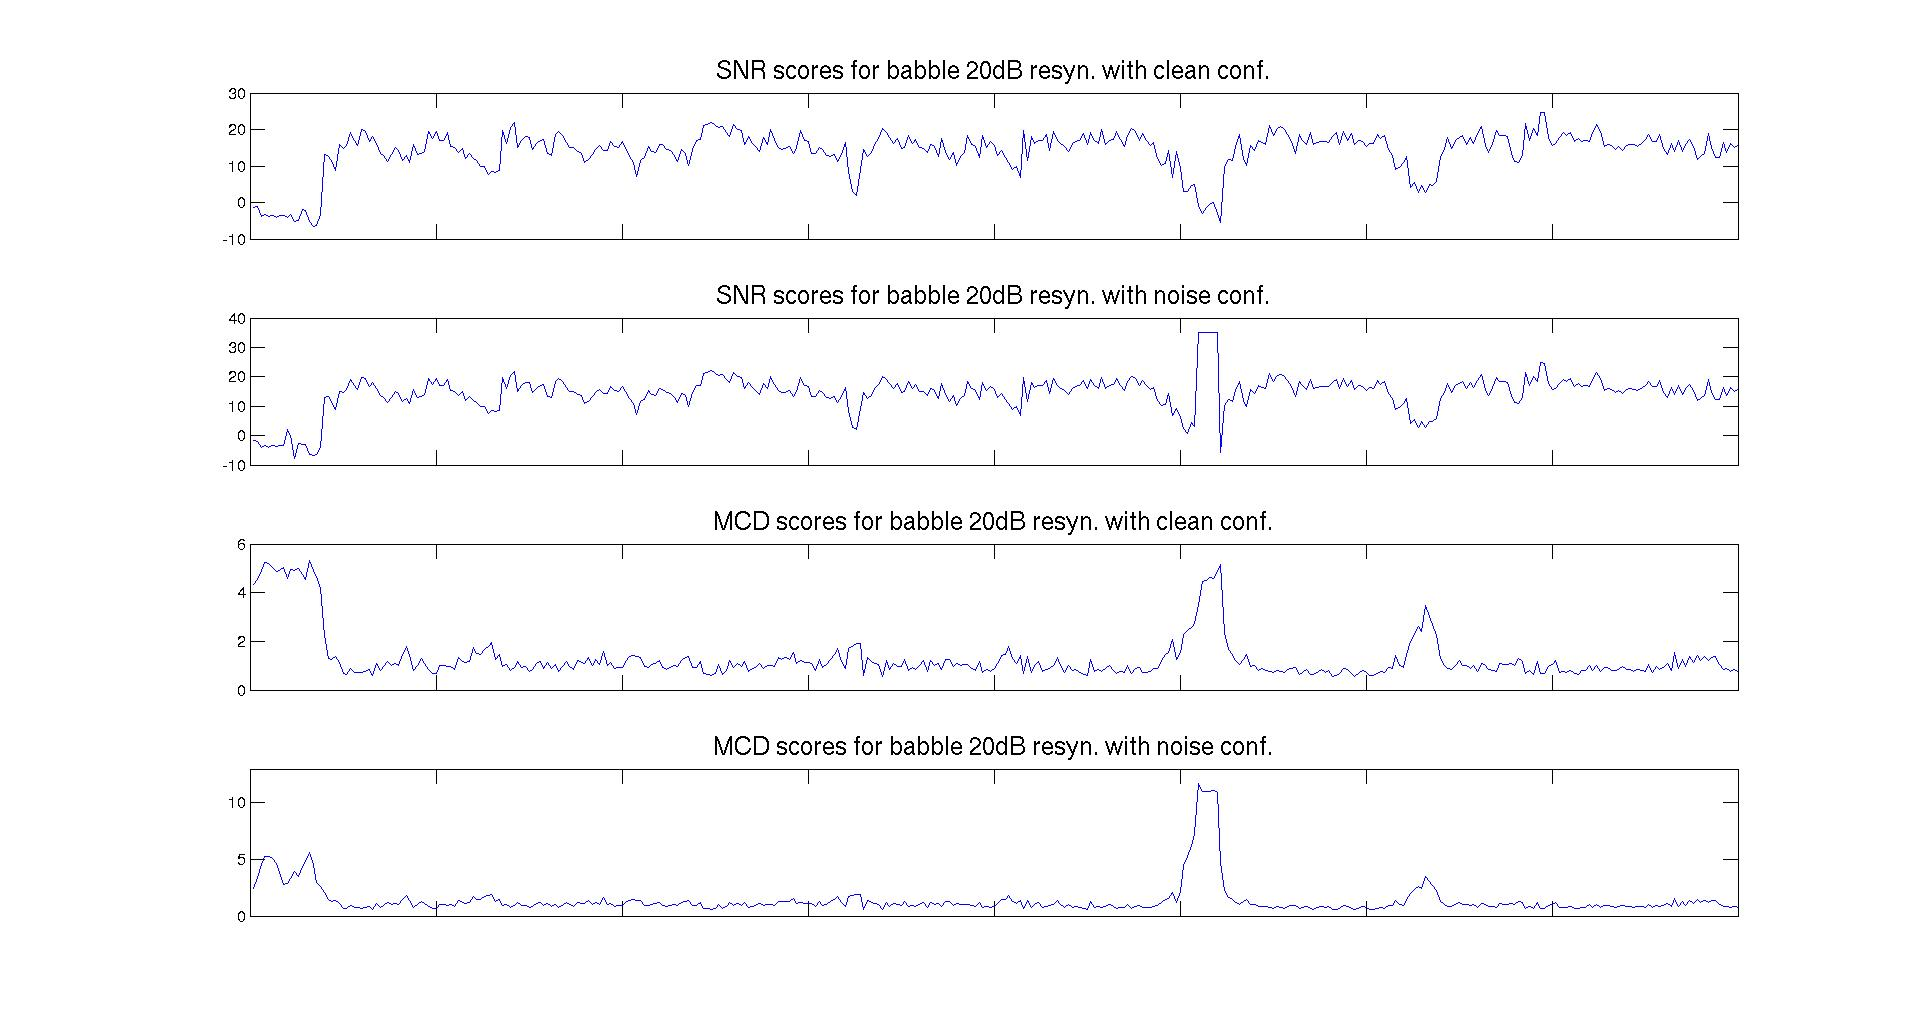
\includegraphics[width=1.3\textwidth]{images/babble20clean_vs_noise.jpg}
\end{adjustwidth}
\caption{SNR and MCD measures of a resynthesized sample with babble 20dB background noise using and not using the noise reduction module (values in Appendix \ref{glott_conf_noise_red}, set to true)}
\label{fig:babble20_clean_vs_noise}
\end{figure}

\subsection{Feature Extraction}
\label{experiments_feature_extraction}
The GlottHMM vocoder includes an analysis module that extract the features from audio files.
%
However, the features extracted with this module are only the static features. 
%
Other features have to be calculated, such as the dynamic features, and in our case, noise robust features could be helpful in the adaptation process.
%
These noise robust features are the Aurora features \cite{etsi202}, calculated with the ETSI advanced front-end.
%
For calculating the rest of the features, the dynamic ones and the Global Variance (GV) \cite{toda2005speech}, used to solve over-smoothing problems, the scripts developed by Antti Suni, from the University of Helsinki, are used.

The final feature vector used in this system is a 183-dimension vector composed by:

\begin{itemize}
	\item 30 LSF components + 1 energy
	\item 10 LSF source
	\item 5 harmonic-to-noise ratio (HNR)
	\item 1  $F_{0}$
	\item 14 Aurora components
\end{itemize}

From all the features except for the Aurora features the scripts used calculate the dynamic features (delta and delta-delta). 
%
The dynamic features for the Aurora are calculated with a snippet of the scripts used that does the delta-calculation.
%
The addition of all the static and dynamic features gives the 183-dimension of the final feature vector.

It must be pointed out that during the training the Aurora features have no function, but they were investigated in \cite{karhila_jstsp_14} together with STRAIGHT features founding out that they improve the alignment when adaptation was not used, reason why they were tested in this project.
%
Unfortunately, no improvement was obtained over the LSF features in the case of the GlottHMM-based system.
%
The system learns about them during the training to be able to adapt according to the noise robustness provided by these features.
%
However, during the experiments it was discovered that adapting with the Aurora features in stead of the LSFs not only does not produce any improvements but the results were clearly poorer.
%
This was obviously noticed after adapting. 
%
Therefore, although the Aurora features are not used at all, they must be calculated in the adaptation data because of the construction of the average voice model, which embodies them in its feature vector composition.

\subsection{Average Voice Model}
\label{experiments_av_voice_model}
As a proper modelling of the glottal pulse has been shown to improve the quality of low $F_{0}$ voices while higher $F_{0}$ ones do not benefit as much (impulse excitation can be adequate for them), we are focusing on male voices.

The average voice model of the speaker-adaptive speech synthesis system built in this work is trained on speech data from the Finnish PERSO corpus, with the features obtained as described in Section \ref{experiments_feature_extraction}.
%
20 male voices from this corpus were used.

To train the model, a modified version of the EMIME 2010 Blizzard Entry \cite{emime_blizzard} was used, using SAT and 3 reclustering iterations, using the configuration for GlottHMM attached in Appendix \ref{glott_conf_file}, where the noise reduction module is not used: clean configuration. 
%
The third iteration gives us the multi-space distribution hidden semi-Markov models (MSD-HSMM) forming the average voice model.

The STRAIGHT voice is trained identically to \cite{karhila_jstsp_14}.

\subsection{Adaptation}
\label{experiments_adaptation}
Once the average voice model trained with high-quality data is ready, we can use the noisy data to adapt to different target speakers.

Three different types of noise were used in this project: Babble, factory and machine gun noise, with different SNR levels.
%
The noisy samples were obtained adding noise from the NOISEX-92 corpus \cite{Varga1993247} to utterances from the EMIME corpus \cite{wester_accent2010}.
%
105 utterances from each of the three target speakers conform the training of the adaptation transforms.

The adaptation transforms are calculated using a combined algorithm with linear regression and MAP adaptation (see \ref{hmm_synthesis_adaptation}).
%
Two rounds of CSMAPLR followed by one round of MAP adaptation conform the combined algorithm.

The regression trees were limited to 64 leaf nodes to obtain robust adaptation transforms, after discovering by trial and error that higher values carried a decrease in the quality of the synthetic speech.
%
Due to the noise present in the data, more data is needed in one node to strengthen the transforms.
%
Moreover, to correct some mistaken phoneme's durations a realignment of the test labels using the average voice model was done prior to the synthesis.

Finally, speech enhancement based on non-negative matrix factorization \cite{raj_interspeech2010} was carried out to test the benefits, if any, obtained.
%
The adaptation procedure with the enhanced data is similar to the noisy cases.

The values of the noise reduction parameters shown in Appendix \ref{glott_conf_noise_red} are the values used in the noise reduction configuration of GlottHMM.
%
When the energy of the frame is below 4.5dB (noise reduction limit) the gain of the frame is reduced by 35dB (noise reduction).

In the adaptation of all the noisy cases the noise reduction configuration is used.
%
Also, adaptation using clean data is done using both the clean configuration and the noise reduction configuration.
%
Using both configurations is done to compare due to the results obtained in Section \ref{experiments_initial}.

\subsection{Synthesis}
\label{experiments_synthesis}
The voices of three different male speakers under different noise conditions were synthesized during this work.
%
The clean and all the noisy cases were synthesized using the $F_{0}$ extracted from each case.
%
However, the problems with its estimation are clearly audible when comparing to the synthesis done with an external $F_{0}$ extracted from the clean data of each speaker.
%
The comparison to the STRAIGHT synthesized speech is done using the external $F_{0}$ synthetic samples obtained with the GlottHMM-based system, focusing on the effects of noise in the spectral components.

Both systems where constructed using the HTK toolkit \cite{young1997htk} and in the case of the GlottHMM-based one, a single, generic pulse was used to produce speech.